\section{Problèmes rencontrés et solutions}

Cette section présente les principales difficultés matérielles et logicielles rencontrées au cours du développement du système d’acquisition radar, ainsi que les solutions mises en œuvre pour y remédier. L’objectif est de garantir une capacité d’acquisition et de sauvegarde fiable des données, condition indispensable à l’exploitation ultérieure de la chaîne de traitement SAR.

\subsection{Problème d’acquisition : impossibilité de sauvegarder les données expérimentales}

\subsubsection{Constat}

L’architecture d’essai initiale repose sur l’utilisation de la carte ST200, associée au logiciel propriétaire \textit{SignalExplorer} fourni par RFBeam. Cette solution offre une prise en main rapide du matériel, grâce à l’intégration d’antennes et de formes d’onde prédéfinies, et facilite ainsi la mise en place de premiers cas de test expérimentaux.

Toutefois, dans la configuration retenue, \textit{SignalExplorer} ne permet pas la sauvegarde des données complexes $I/Q$ associées à la forme d’onde utilisée. Cette limitation empêche toute exploitation des mesures réalisées et compromet directement la mise en œuvre de la chaîne de traitement radar envisagée.
Cette limitation a conduit à l’examen de deux hypothèses. La première concerne une éventuelle insuffisance du débit de communication USB entre la carte et l’ordinateur hôte. Cette hypothèse a été rapidement écartée, les ordres de grandeur requis pour l’acquisition restant très inférieurs aux capacités offertes par un bus USB~2.0.  

La seconde hypothèse, finalement retenue, attribue la limitation à une contrainte purement logicielle.

\subsubsection{Solution mise en place}

La solution adoptée consiste à contourner la surcouche logicielle fournie par RFBeam en développant une application d’acquisition dédiée, reposant sur une API Python et s’appuyant directement sur les pilotes National Instrument. Cette approche permet de reprendre le contrôle complet de la chaîne d’acquisition, tant sur le format des données enregistrées que sur l’organisation temporelle des mesures.

Elle garantit en particulier l’accès aux données $I/Q$ brutes, leur structuration conforme aux besoins du traitement SAR (organisation en temps rapide et temps lent), ainsi qu’une compatibilité directe avec les algorithmes de compression en distance et de formation d’image mis en œuvre en parallèle.

\subsection{Développement de la solution Python d’acquisition et de pré-traitement}
\label{sub:ihm}

\subsubsection{Objectifs}

Le développement de la solution d’acquisition en Python vise à fournir un outil stable et reproductible, configurable en termes de fréquence d’échantillonnage, de durée d’acquisition et de mode de déclenchement. L’outil doit également permettre le pilotage de la commande d’émission, en particulier la génération de rampes FMCW, et assurer le stockage des données $I/Q$ dans un format directement exploitable par la chaîne de traitement SAR. Enfin, cette solution est conçue de manière à rester compatible avec une évolution vers un capteur embarqué sur une plateforme en mouvement.

\subsubsection{Implémentation}

La mise en œuvre de cette solution a nécessité, dans un premier temps, l’installation des pilotes associés à la carte National Instruments intégrée au ST200, disponibles sur le site du constructeur. Une fois ces dépendances installées, les bibliothèques Python nécessaires ont été déployées, en particulier celles permettant l’accès à l’API NI-DAQ ainsi que la gestion de l’interface graphique.

Le fonctionnement du logiciel \textit{SignalExplorer} a ensuite été reproduit en Python, incluant la génération de la forme d’onde, l’affichage dynamique des signaux acquis et, surtout, l’ajout d’une fonctionnalité dédiée à la sauvegarde systématique des données $I/Q$ pour un traitement ultérieur.
\begin{figure}
    \centering
    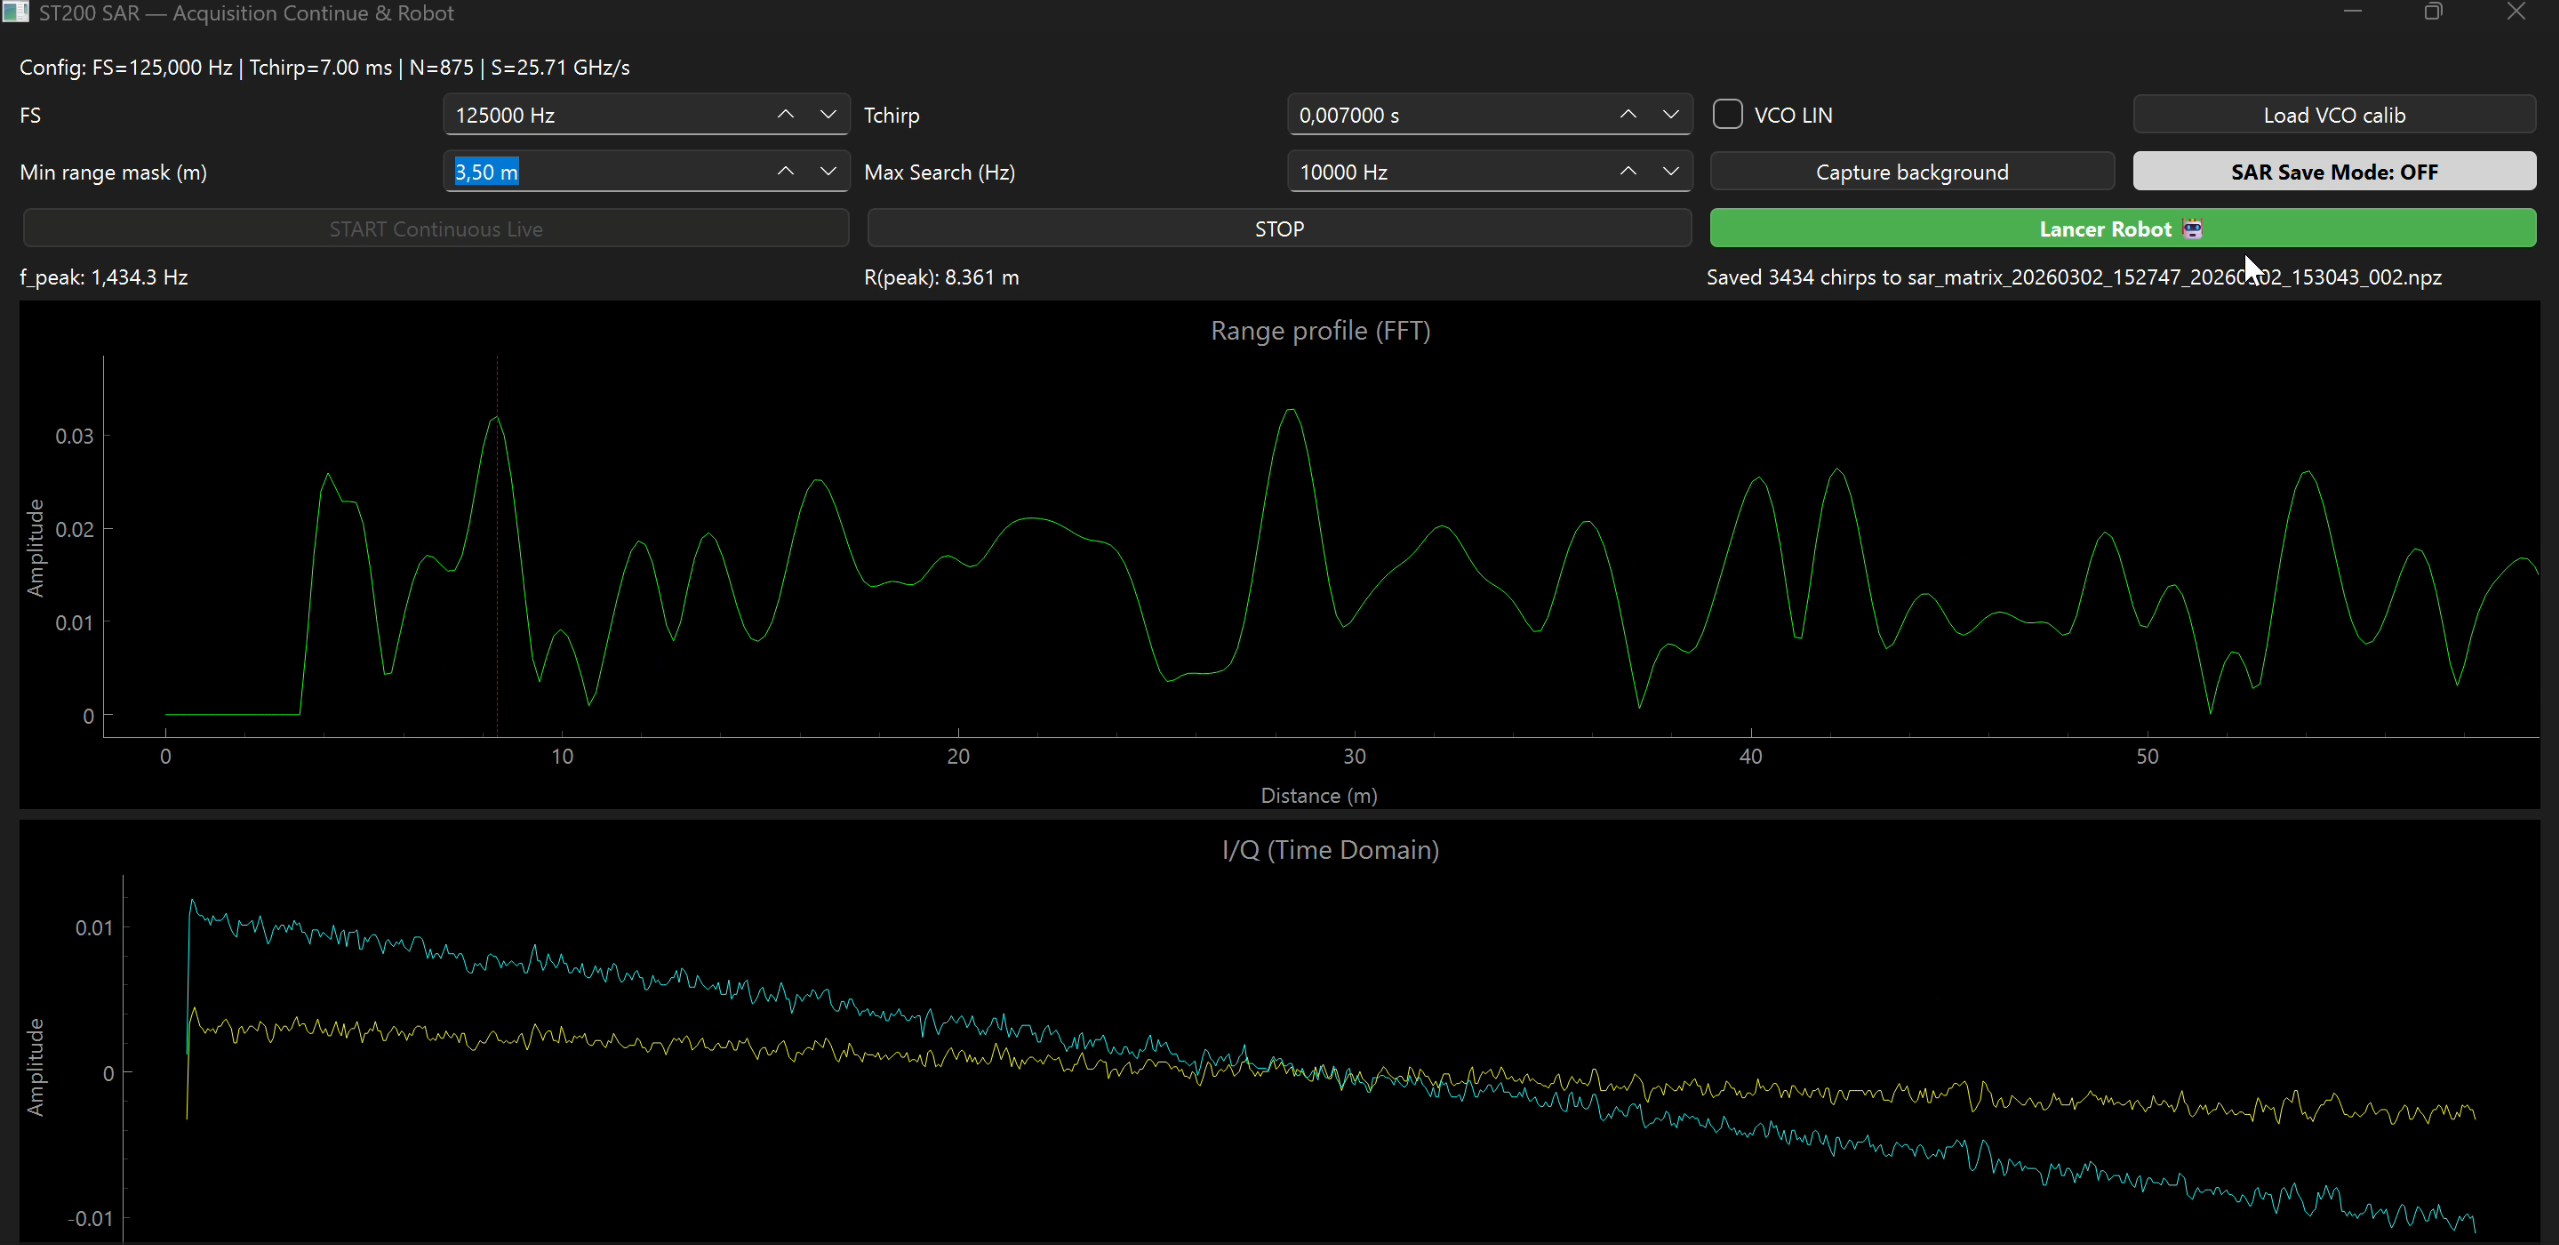
\includegraphics[width=1\linewidth]{src/rapport_complet/img/IHM_developpée.png}
    \caption{Interface graphique du logiciel développé}
    \label{fig:IHM_developpée}
\end{figure}

\subsubsection{Impacts projet}

Cette évolution permet de disposer de données expérimentales exploitables hors ligne et d’un contrôle fin sur l’ensemble de la chaîne d’acquisition. En contrepartie, elle implique un effort de développement supplémentaire lié à la reprogrammation de fonctionnalités initialement prises en charge par le logiciel propriétaire, ainsi qu’à la validation de la stabilité et de la reproductibilité de l’outil développé.
Le programme développé à permis de mettre en évidence un problème qui n'avait pas encore été découvert. 

\subsection{\emph{Self-mixing} : contrainte sur l’expérimentation}

\subsubsection{Nature du problème}

Les essais expérimentaux ont mis en évidence une limitation liée au phénomène de \textbf{self-mixing}, également désigné comme auto-mélange ou fuite directe du signal d’émission vers la réception. Une fraction du signal émis est directement couplée à la voie de réception, générant une composante dominante susceptible de masquer les échos utiles lorsque les conditions expérimentales ne sont pas favorables.

\subsubsection{Visualisation expérimentale du phénomène}

Le phénomène de self-mixing se manifeste clairement sur le profil de distance obtenu après application d’une transformée de Fourier rapide (FFT) au signal. La Figure~\ref{fig:self_mixing_range} présente un exemple représentatif de profil mesuré.

On y observe une composante d’amplitude très élevée dans les premières cellules de distance, proches de l’origine. Cette contribution ne correspond pas à un écho issu d’une cible réelle, mais à une fuite directe du signal d’émission vers la réception. Elle se traduit par une énergie dominante à très basse fréquence de battement, interprétée par le traitement comme une cible située à très courte distance.

Cette composante parasite monopolise la dynamique du profil de distance et masque les éventuels échos utiles situés à plus grande distance. En pratique, les premières cellules de distance deviennent inexploitables, ce qui impose une distance minimale à partir de laquelle les retours peuvent être distingués du bruit et de la fuite directe.

\begin{figure}[H]
  \centering
  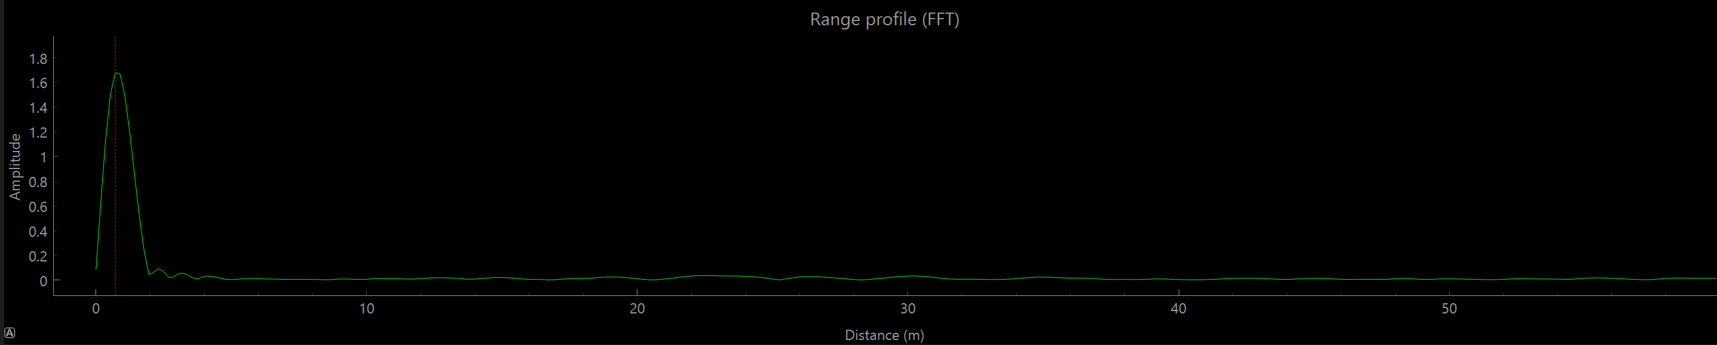
\includegraphics[width=1\textwidth]{src/rapport_complet/img/self_mixingIHM.png}
  \caption{Profil de distance obtenu après FFT illustrant le phénomène de self-mixing.}
  \label{fig:self_mixing_range}
\end{figure}

\subsubsection{Conséquences sur les tests}

Cette contrainte se traduit par plusieurs limitations expérimentales. Elle impose tout d’abord un espace minimal pour la réalisation des essais, compatible avec la distance minimale de l’ordre de 5~m mise en évidence expérimentalement. Elle restreint également la géométrie de scène admissible, notamment en termes de distance, d’angle de visée et de surface illuminée. Enfin, elle nécessite une adaptation du protocole expérimental afin d’éviter les configurations dans lesquelles la fuite directe domine la dynamique du signal.


\paragraph*{Conclusion}

La résolution des problématiques de limitations logicielles constitue une étape essentielle dans la mise au point du système expérimental. Le dispositif d’acquisition étant désormais fonctionnel et les principales contraintes identifiées, les travaux peuvent se poursuivre avec la mise en place de l’intégration mécanique du capteur et la préparation des campagnes de tests expérimentaux.

